
\def\stringseashells{S,h,e,\_,s,e,l,l,s,\_,s,e,a,s,h,e,l,l,s,\_,b,y,\_,t,h,e,\_,s,e,a,s,h,o,r,e}
\def\stringstruggled{I, ,s,t,r,u,g,g,l,e,d, ,t,o, ,m,a,k,e, ,t,h,i,s, ,f,i,g,u,r,e, ,w,i,t,h, ,t,i,k,z,!}


\begin{frame}{\textcolor{gray}{Sketch-based approaches to process massive \bblue{string data}}}
    \pause
    A string $T$ of length $n$ is a sequence $T[0]T[1]...T[n-1]$ of characters from a finite alphabet $\Sigma$ of size $\sigma$.\pause \\
    \begin{center}
        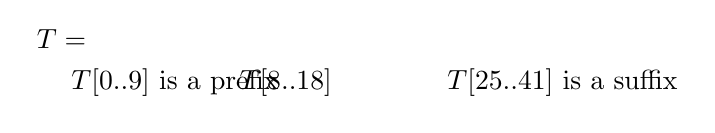
\begin{tikzpicture}[x = 2em]
            \node (t) at (-0.8,0) {\smash{$T=$}$\vphantom{m}$};
            \numberedstring{\stringstruggled}
            \onslide<4|handout:0>{
                \numberedsubstring[blue]{\stringstruggled}{8}{18}
                \node at (13*0.25,-0.5) {$T[8..18]$};
            }
            \onslide<5>{
                \numberedsubstring[blue]{\stringstruggled}{0}{9}
                \node at (5*0.25,-0.5) {$T[0..9]$ is a prefix};
            }
            \onslide<6>{
                \numberedsubstring[blue]{\stringstruggled}{25}{42}
                \node at (33*0.25,-0.5) {$T[25..41]$ is a suffix};
            }
        \end{tikzpicture}
        \\
    \end{center}
    \pause
    \textbf{Definitions and Notations}\\
    The \textbf{substring} from position $i$ to position $j$: $T[i]T[i+1]...T[j]$ is denoted $T[i..j]$.\\ \pause
    Substrings of the form $T[0..j]$ are \textbf{prefixes}.\\ \pause
    Substrings of the form $T[i..n-1]$ are \textbf{suffixes}.\\ \pause

    \medskip
    In every algorithm in the presentation we assume \ntheme{the word RAM model} with word of length logarithmic in the size of the input.
\end{frame}

\begin{frame}{\textcolor{gray}{Sketch-based approaches to process massive \bblue{string data}}}
    
    \small
    % any file can be seen as a string. 
    %\pause
    Strings are used in fields such as \bgreen{Bioinformatics}, \bblue{Information Retrieval}, and \borange{Cyber-security}.\pause

    \medskip
    \begin{tabular}{l  c c c c}
        \emph{Strings} & Binary file & DNA sequence & ASCII string file & UTF-8 string file \\
        \rule{0pt}{10ex}    
        &
        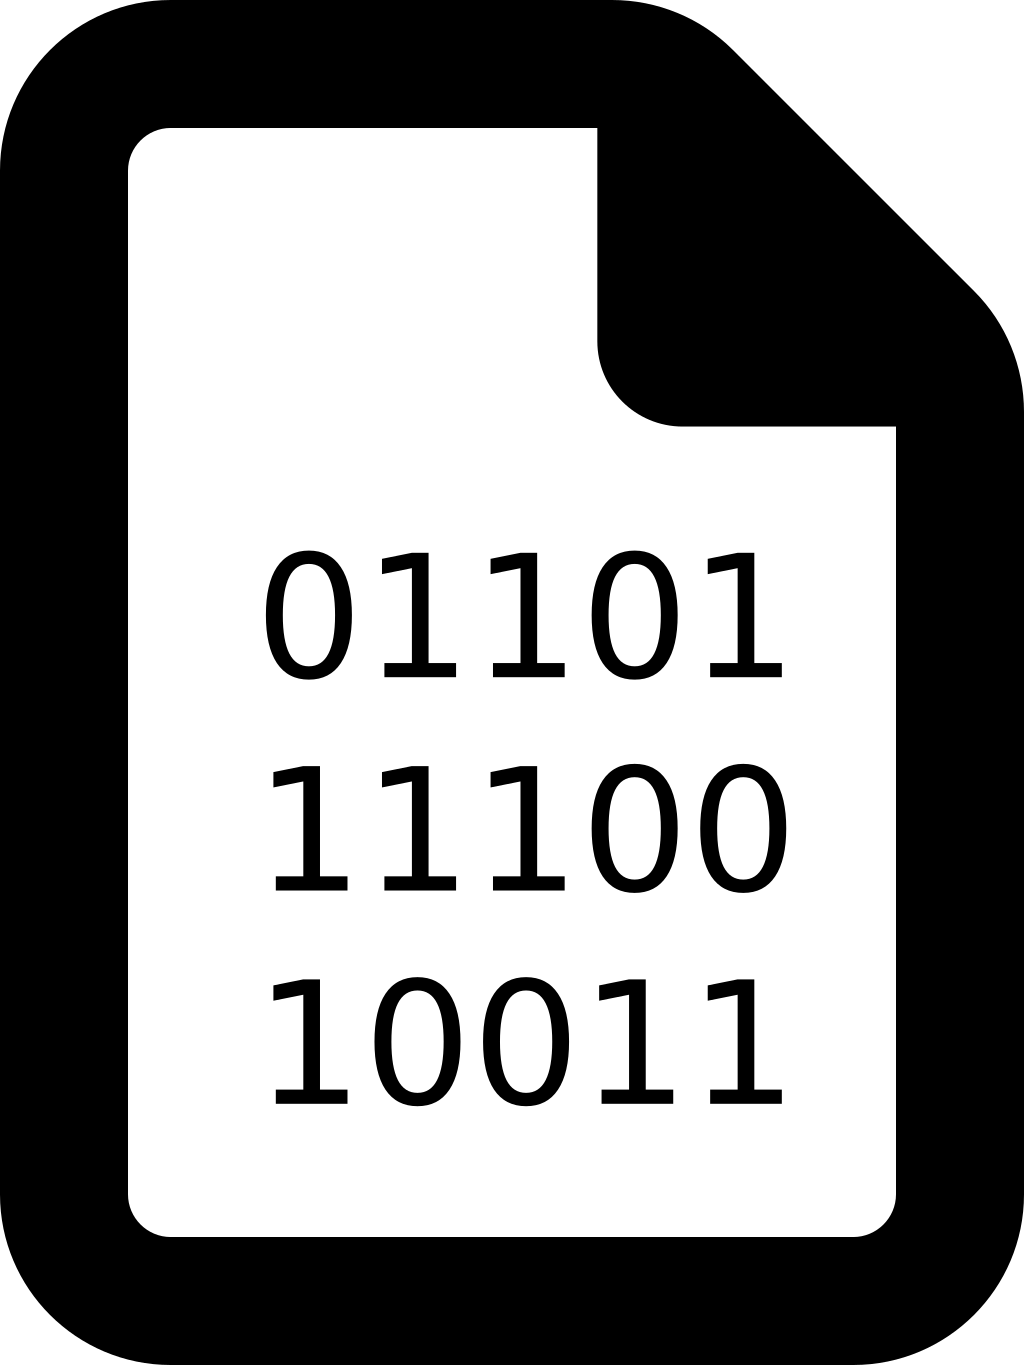
\includegraphics[width=1cm]{pictures/file-bin.png}&
        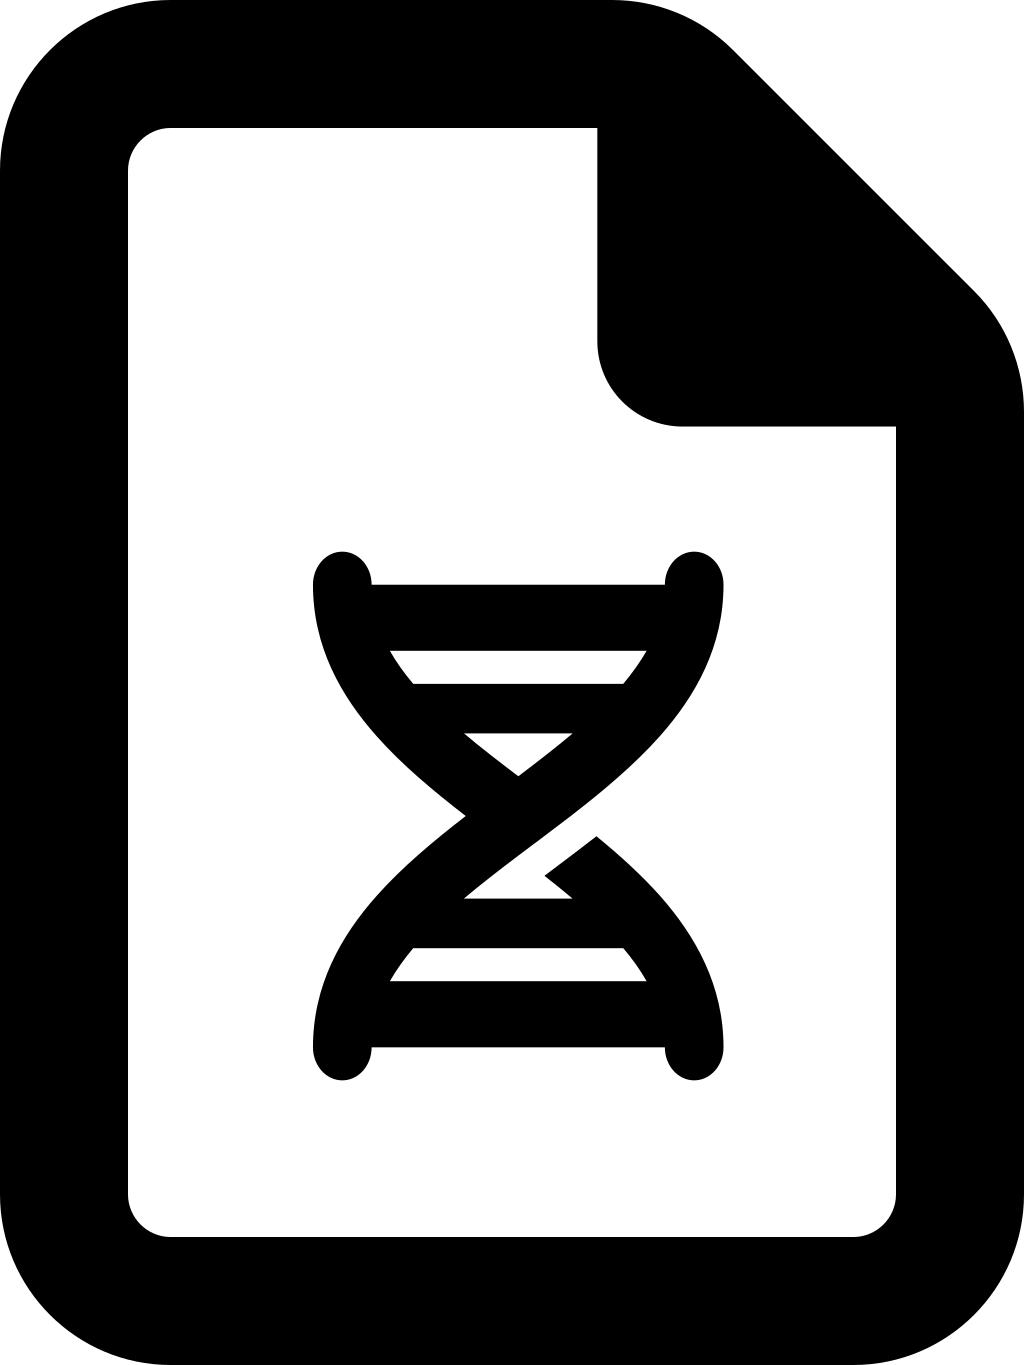
\includegraphics[width=1cm]{pictures/file-dna.png}&
        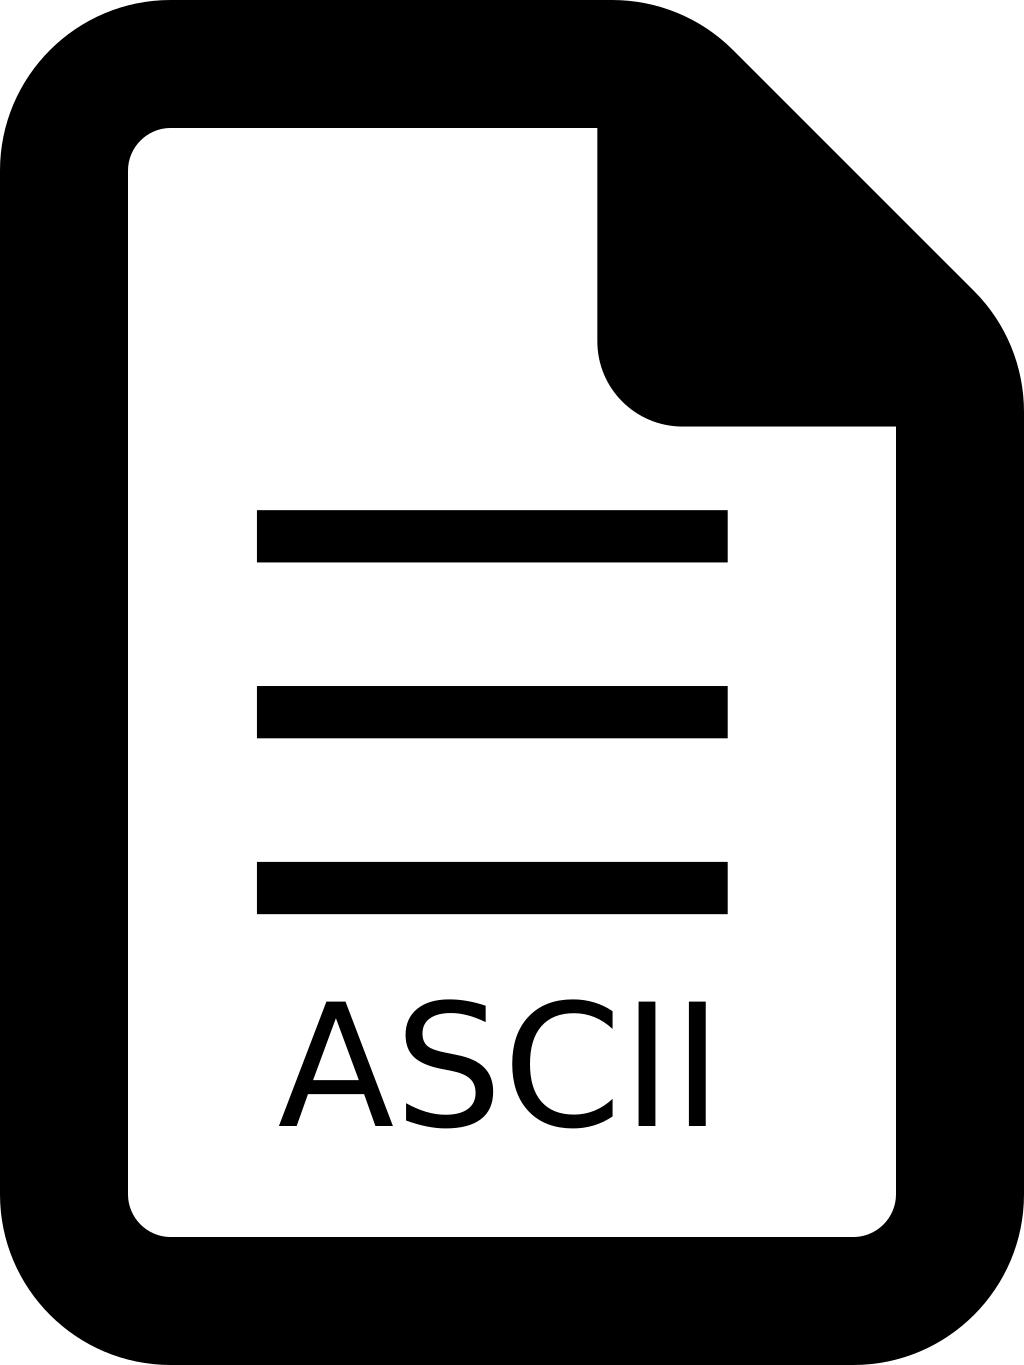
\includegraphics[width=1cm]{pictures/file-ascii.png}&
        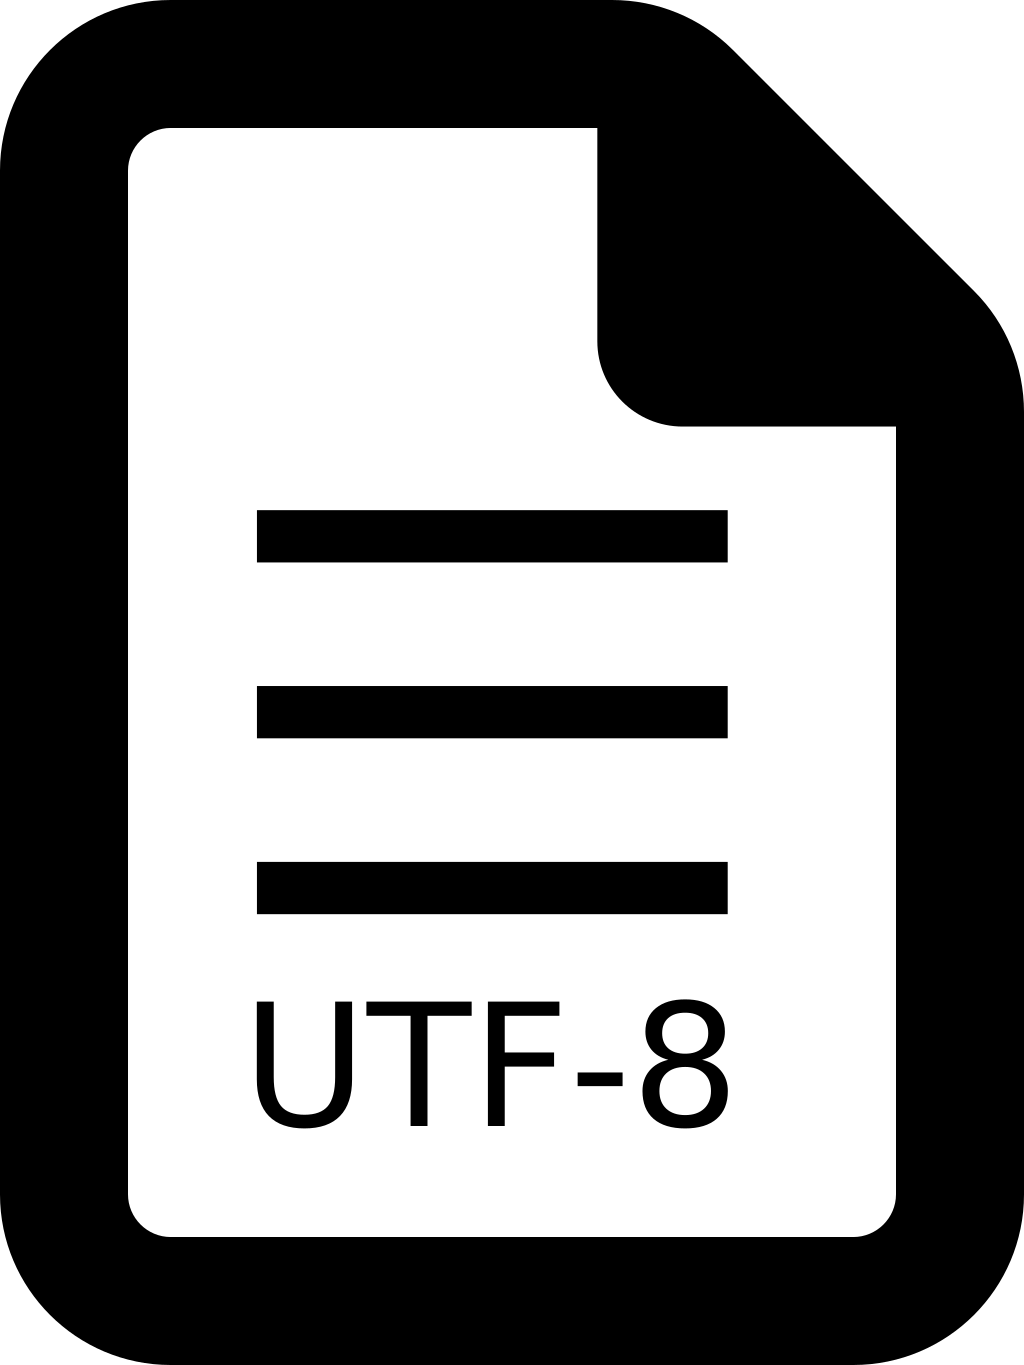
\includegraphics[width=1cm]{pictures/file-utf-8.png}
        \\
        \rule{0pt}{4ex}  
        \emph{Alphabets} & $\Sigma=\{0,1\}$ & $\Sigma=\{\texttt{A,T,C,G}\}$ & $\Sigma=\{0,\dots , 127\}$ & $\Sigma = \{0, \dots, 1~112~063\}$\\
    \end{tabular}\pause
    \bigskip

    \textbf{Classical task:} \pause Given a pattern $P =$ \texttt{th}, does it occur in  $T$ and where?
    
    \begin{center}
        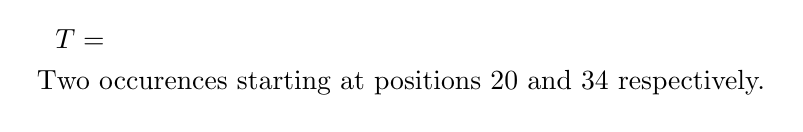
\begin{tikzpicture}[x = 2em]
            \node (t) at (-0.8,0) {\smash{$T=$}$\vphantom{m}$};
            \numberedstring{\stringstruggled}
            \numberedsubstring[myorange]{\stringstruggled}{20}{21}
            \numberedsubstring[myblue]{\stringstruggled}{34}{35}
            \onslide<4->{
                \node at (20*0.25,-0.5) {
                    Two occurences starting at positions \borange{20} and \bblue{34} respectively.
                };
            }
        \end{tikzpicture}
        \\
    \end{center}

\end{frame}

\begin{frame}{\textcolor{gray}{Sketch-based approaches \borange{to process} massive string data}}
\pause
\ntheme{Three main types of tasks in this thesis:}\\ \pause
\fbox{
\begin{minipage}[t][6cm][t]{0.3\textwidth}
    \begin{center}
        \vspace{0.2cm}
        \btheme{Complex matching}
        \vfill
        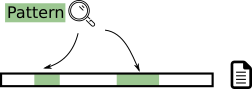
\includegraphics[width=0.8\textwidth]{pictures/complex.png}
    \end{center}
    \vfill
    Examples:
    \begin{itemize}
        \item Regular expressions
        \item Wildcards
        \item Degenerate
        \item ... 
    \end{itemize}
    \vspace{0.3cm}
\end{minipage}}\pause
\hfill
\fbox{
\begin{minipage}[t][6cm][t]{0.3\textwidth}
    \begin{center}
        \vspace{0.2cm}
        \btheme{Similarity measures}\\
        \btheme{and distances}
        \vfill
        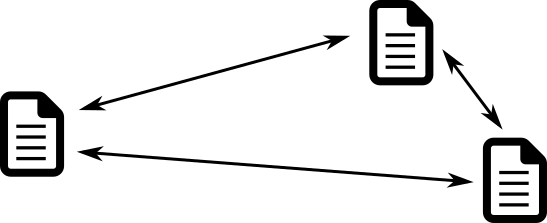
\includegraphics[width=0.7\textwidth]{pictures/dist.png}
    \end{center}
    \vfill 
    Examples:
    \begin{itemize}
        \item Hamming distance
        \item LCS
        \item Edit distance
        \item ...
    \end{itemize}
    \vspace{0.3cm}
\end{minipage}}\pause
\hfill
\fbox{
\begin{minipage}[t][6cm][t]{0.3\textwidth}
    \begin{center}
        \vspace{0.2cm}
        \btheme{Repetitions detection}
        \vfill
        
\includegraphics[width=0.9\textwidth]{pictures/repet.png}
    \end{center}
    \vfill
    Examples:
    \begin{itemize}
        \item Periods
        \item Squares 
        \item Runs
        \item ...
    \end{itemize}
    \vspace{0.3cm}
\end{minipage}}
\end{frame}

% Coin Coin COin
\begin{frame}{\textcolor{gray}{Sketch-based approaches to process \bred{massive} string data}}

    {\small Strings are used in fields such as \bgreen{Bioinformatics}, \bblue{Information Retrieval}, and \borange{Cyber-security}.}
    \begin{center}
        \pause
        \begin{tabular}{l c c c c}
            Data type & \textcolor{black!10!myblue}{Webpage} &  \textcolor{black!10!mygreen}{E. coli genome} & \textcolor{black!10!myorange}{Software repository} & \textcolor{black!10!mygreen}{Human genome}\\ \hline
            Size & $\sim$ 2 Mb & $\sim$ 5Mb &  $<$ 1 Gb & $\sim$ 3 Gb 
        \end{tabular}\pause

        \bigskip

        \begin{tabular}{l c c c}
            Archive & \textcolor{black!10!myorange}{Software Heritage} & \textcolor{black!10!mygreen}{European Nucleotide (ENA)} & \textcolor{black!10!myblue}{Wayback Machine}  \\ \hline
            Size & $>$ 1 Pb & $>$ 50 Pb &  $>$ 70 Pb
        \end{tabular}
    \end{center}\pause

    \bigskip
    Many datasets of intermediate size: Tara ocean, 661K bacterial genome from ENA...\pause

    \bigskip

    Queries with a \textbf{high complexity} in time or space \textbf{cannot scale to large datasets}. \pause

    \bigskip

    But some part of the data can be \btheme{redundant} or \btheme{not needed} for the queries we want?\pause

\end{frame}

\begin{frame}{\textcolor{gray}{\bgreen{Sketch-based} approaches to process massive string data}}
    \pause
    \begin{columns}
        \column{.6\textwidth}
        A \textbf{sketch} is a \bblue{lossless} or \borange{lossy} compression that \textbf{keeps only the essential characteristic of the input} needed to answer a specified type of query.\\
        \column{.35\textwidth}
        
\includegraphics[width=1.8cm]{pictures/photo_betisou.jpg}
        \hspace{0.5cm}
        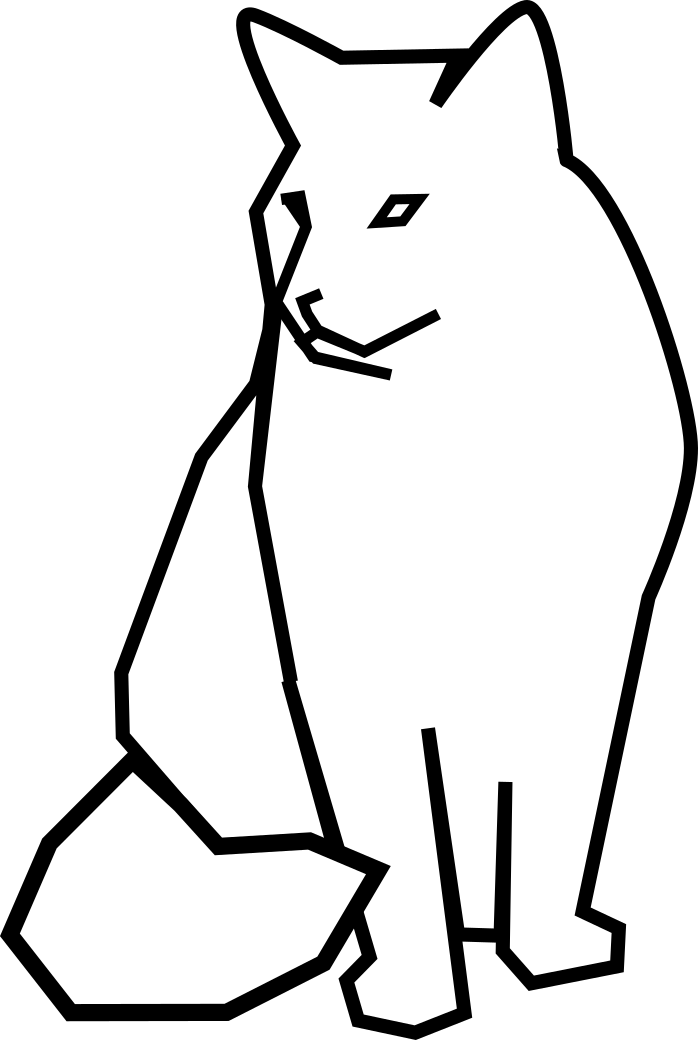
\includegraphics[width=1.8cm]{pictures/betisou.png}\\
        \begin{center}
            "Is this a cat?"
        \end{center}
    \end{columns}
    \pause

    {\Large Examples:}
    \medskip
    \begin{columns}
        \column{.01\textwidth}
        \column{.48\textwidth}
        {\borange{Lossy: Karp--Rabin fingerprints}}
        \column{.48\textwidth}
        {\bblue{Lossless: Lempel--Ziv factorization}}
    \end{columns}
    
\end{frame}

\begin{frame}{Example of lossy sketch: Karp--Rabin fingerprints}
    \pause
    \begin{columns}
        \column{0.6\textwidth}
        A hash function $\varphi$ such that,\\ 
        for two string $X$ and $Y$ with $|X|=|Y|$: 
        \begin{itemize}
            \item If $X=Y$, then $\varphi(X)=\varphi(Y)$. 
            \item If $\varphi(X)=\varphi(Y)$ then the strings match w.h.p. and it can be tested in $\Oh(1)$ time.
        \end{itemize} 

        \column{0.35\textwidth}
        \vspace{-1cm}
        \begin{mydefblock}{\footnotesize \textcolor{gray}{Karp--Rabin fingerprints}}
            \beamermathcolor{gray}
            \scriptsize
            For $p>|\Sigma|$ a prime and $b > |\Sigma|$,
            the fingerprint of a string $P$ of length $m$ is:
            \begin{equation*}
                \resizebox{\hsize}{!}{$\varphi_{p,b}(P) = \mathop{\sum}_{i = 0}^{m-1}  P[i]b^{m-i-1} \bmod p$}
            \end{equation*}
            \vspace{-0.5cm}
        \end{mydefblock}
    \end{columns}\pause

    Occupies constant space, but we cannot reconstruct the original strings.\\ \pause
    \smallskip
    Given $X$, we can compute $\varphi(X)$ in $\Oh(|X|)$ time.\\ \pause
    \medskip

    \begin{columns}
        \column{0.5\textwidth}
        \btheme{Rolling hash function}\\ 
        For a string $T$ and $i<j$, given $\varphi(T[i..j])$, $T[i]$ and $T[j+1]$,
        we can compute $\varphi(T[i+1..j+1])$ in $\Oh(1)$ time.
        \column{0.4\textwidth}
        
\includegraphics[width=\textwidth]{pictures/slidding_window.png}
    \end{columns}
\end{frame}

\begin{frame}{Example of lossless sketch: Lempel--Ziv  factorization}

    \ntheme{Decomposition in phrases:} $T = f_1f_2\dots f_z$, (LZ76 with overlap version)\\
    \onslide<3->{The unique LZ-phrase starting at position $s$, $f_i=T[s..e]$ is such that $T[s..e]$ is the longest prefix of $T[s..n-1]$ that has a previous occurrence in $T[0..e]$.}
    \vspace{.5\baselineskip}
    
    \onslide<2->{
    \begin{center}
    \begin{overlayarea}{\textwidth}{2.5cm}
    \begin{tikzpicture}
    \tikzset{barcolor/.style={black, densely dotted}}
    \tikzset{fcolor/.style={black}}
    
    \setcounter{symbid}{0}
    \foreach[count=\factorid from 1, evaluate=\factorid as \prevfid using int(\factorid-1)] \factorset in {%
    {a},
    {b},%
    {c},
    {b,a},
    {b,a,a},
    {b,c,b,a,c},%
    {b,a,b,a,a,b,c,z},%
    {z,b},
    {a,b,a}%
    }
    {

        \only<3->{
        \ifnum\factorid=7
            \tikzset{barcolor/.style={black, densely dotted}}
            \tikzset{fcolor/.style={black, font=\boldmath}}	
        \else
            \beamermathcolor{black!30!white}
            \tikzset{barcolor/.style={black!20!white, densely dotted}}
            \tikzset{fcolor/.style={barcolor}}
        \fi}

        \path (\thesymbid\lzspacing+0.5\lzspacing, -0.5em) node (leftbar) {};
        \foreach \tsymb in \factorset {
            \addtocounter{symbid}{1}
            \node[inner sep=0] (\thesymbid) at (\thesymbid\lzspacing,0) {\smash{\texttt{\tsymb}\vphantom{$\strut$}}$\vphantom{m}$};
            %\node at (\thesymbid\lzspacing,1) {$\scriptstyle\thesymbid$};
        }
        \path (\thesymbid\lzspacing+0.5\lzspacing, -0.5em) node (rightbar) {};
        \path (leftbar) to node[midway] (centerbar) {} (rightbar);
        %\node[above of=centerbar, fcolor] (flab\factorid) {$f_{\factorid}$};
        \node[above=.75em of centerbar |- \thesymbid.north, fcolor] (flab\factorid) {$f_{\factorid}$};

        \ifodd\factorid\else
            \draw[thick, barcolor] (leftbar.center) to ++(0,1);
            \draw[thick, barcolor] (rightbar.center) to ++(0,1);
        \fi
    }

    \tikzset{hlbox/.style={draw, ultra thick, inner xsep=2.5pt}}

  
    
    \foreach[count=\i from 14, evaluate=\i as \j using int(\i-10)] \x in {b,a,b,a,a,b,c} {
    \node<4->[below=1em of \i, inner sep=0] (low\i) {\smash{\texttt{\x}\vphantom{$\strut$}}$\vphantom{m}$};
    \node<5->[below=1em of \j, inner sep=0] (low\j) {\smash{\texttt{\x}\vphantom{$\strut$}}$\vphantom{m}$};
    }

    \only<4->{
        \node[hlbox, fit=(low14)(low20), myblue] (ma) {};

        \node[below=0 of ma] (malab) {\bblue{already seen}};

    }
    \node<5->[hlbox, fit=(low4)(low10), myblue] (fi) {};

    
    \node<6->[below=1em of 21, inner sep=0] (low21) {\smash{\texttt{z}\vphantom{$\strut$}}$\vphantom{m}$};
    \node<6->[below=1em of 11, inner sep=0] (low11) {\smash{\texttt{b}\vphantom{$\strut$}}$\vphantom{m}$};
    \node<6->[hlbox, fit=(low21), myorange] {};
    \node<6->[hlbox, fit=(low11), myorange] {};

    \only<7->{
        \node[below right=0.3em of fi.south west] (start) {};
        \node[below left=0.3em of ma.south west] (end) {};
        \node[fit=(start)(end), inner sep=0pt] (mlarrowl) {\rightarrowfill};
        \node[fit=(start)(end), inner sep=0pt] (mlarrowr) {\leftarrowfill};
        \node[below=-.65em of mlarrowl] {$d$};
    }    
    \draw node[left=0 of 1] {$T = \strut$};
    \end{tikzpicture}
    \end{overlayarea}
    \end{center}}

    \onslide<8->{Used for \btheme{compression} by representing $f_i=T[s..e]$ by $(d,e-s,T[e])$.}
    \onslide<9->{In the worst case, no compression, but very efficient in practice.}
\end{frame}

\begin{frame}{What is a sketch?}
    \begin{columns}
        \column{.6\textwidth}
        A \textbf{sketch} is a \bblue{lossless} or \borange{lossy} compression that \textbf{keeps only the essential characteristic of the input} needed to answer a specified type of query.\\
        \column{.35\textwidth}
        
\includegraphics[width=1.8cm]{pictures/photo_betisou.jpg}
        \hspace{0.5cm}
        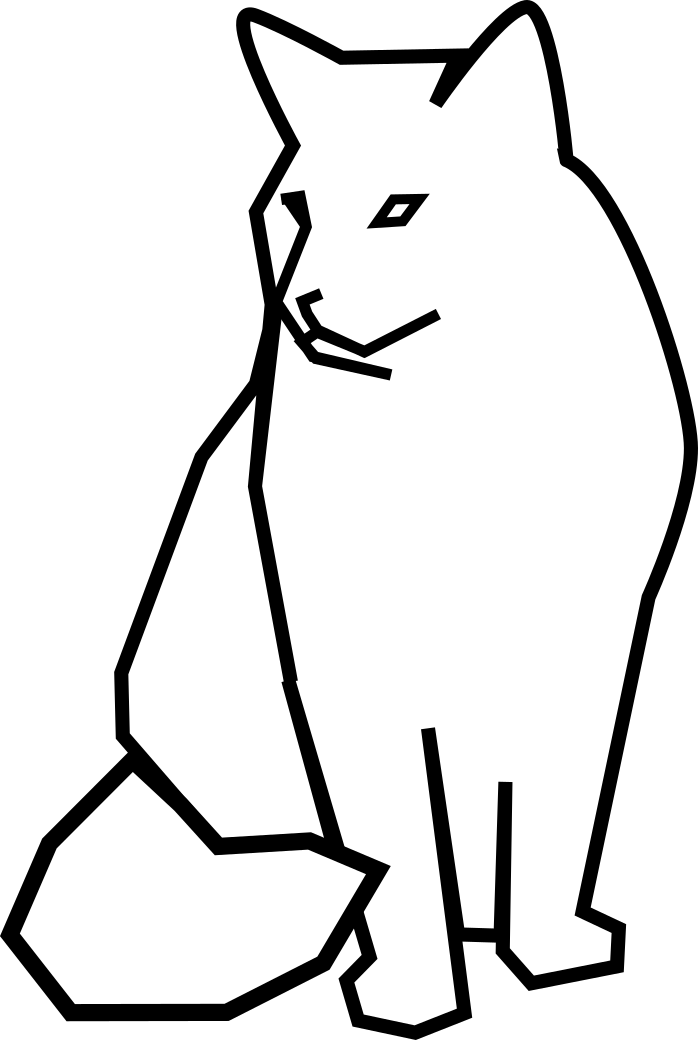
\includegraphics[width=1.8cm]{pictures/betisou.png}\\
        \begin{center}
            "Is this a cat?"
        \end{center}
    \end{columns}

    {\Large Examples:}
    \medskip
    \begin{columns}
        \column{.01\textwidth}
        \column{.48\textwidth}
        {\borange{Lossy: Karp--Rabin fingerprints}}
        \begin{itemize}
            \item They occupy constant space,  
            \item can check whether two strings match with high probability,
            \item but cannot be used to reconstruct the original string. 
        \end{itemize}
        \column{.48\textwidth}
        {\bblue{Lossless: Lempel--Ziv factorization}}
        \begin{itemize}
            \item It is a very efficient compression in practice (used in \texttt{.png} or \texttt{.zip}),
            \item can reconstruct the original string,
            \item but in the worst case it does not compress. 
        \end{itemize}
    \end{columns}
    
\end{frame}

\begin{frame}{Why and how do we use sketches?}
    Sketches are typically much \bgreen{smaller}, thus are promising for \bgreen{scaling to larger} datasets.
    
    \bigskip
    \pause


    \hspace{-0.5cm} {\large \textcolor{black!30!blue}{Two main approaches in this thesis:}}\\
    \begin{columns}
        \column{0.33\textwidth}
        \begin{framed}
            \begin{center}
                \textbf{Sketch as input}\\
                \medskip
                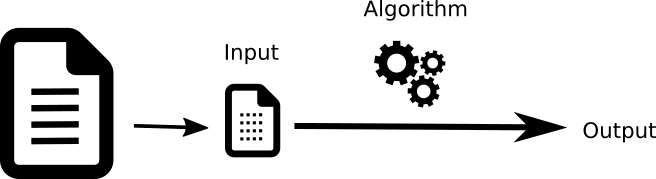
\includegraphics[width=0.95\textwidth]{pictures/sketch_as_input.png}
            \end{center}
            Operating directly on the sketch given as input (not decompressing).
        \end{framed}
        \column{0.66\textwidth}
        \begin{framed}
            \begin{center}
                \textbf{Sketch as you go}\\
                \smallskip
                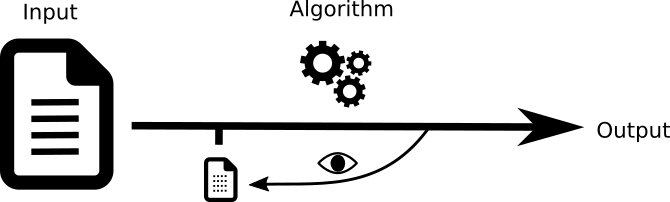
\includegraphics[width=0.5\textwidth]{pictures/sketch_as_we_go.png}
            \end{center}
            Compute the sketch of the input on the fly and use it later on in your algorithm. 
            \begin{itemize}
                \item For streaming
                \item For approximation
            \end{itemize}
        \end{framed}
    \end{columns}
\end{frame}
